\documentclass[tikz,border=10pt]{standalone}
\begin{document}
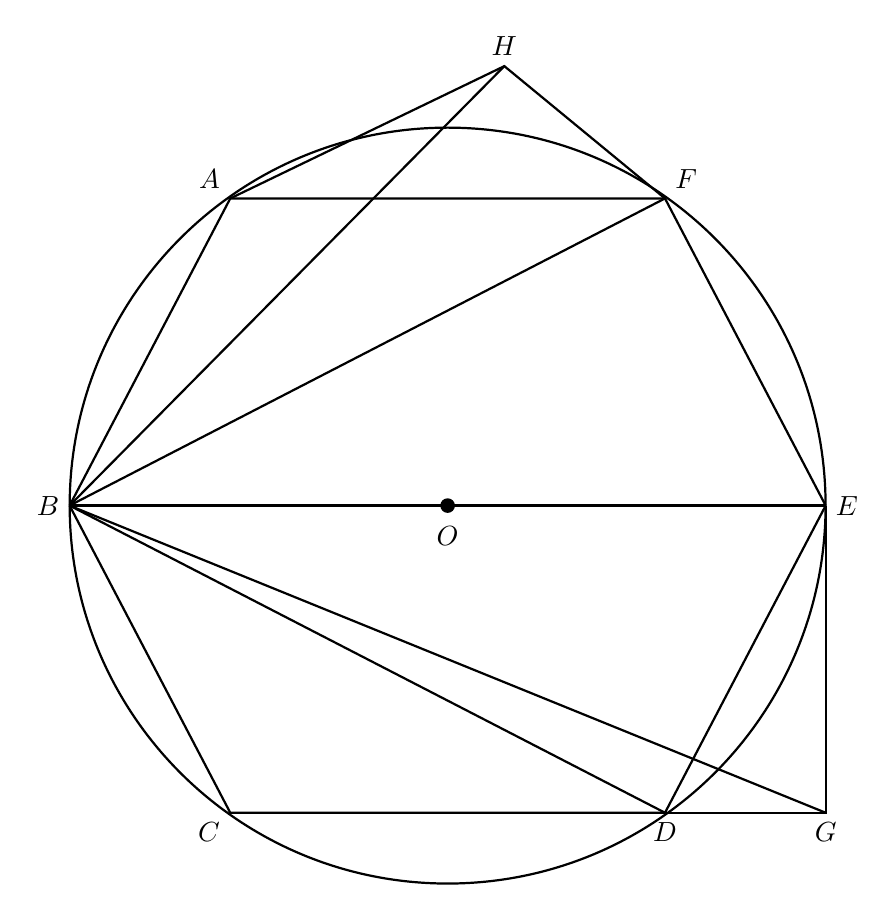
\begin{tikzpicture}[scale=1.2,thick]
\coordinate (O) at (0,0);
\coordinate (B) at (-4,0);
\coordinate (E) at (4,0);
\coordinate (A) at (-2.3,3.25);
\coordinate (F) at (2.3,3.25);
\coordinate (C) at (-2.3,-3.25);
\coordinate (D) at (2.3,-3.25);
\coordinate (G) at (4,-3.25);
\coordinate (H) at (0.6,4.65);

\draw (O) circle (4);
\draw (B) -- (E);
\draw (B) -- (A) -- (F) -- (E);
\draw (B) -- (F);
\draw (A) -- (H) -- (F);
\draw (B) -- (H);
\draw (B) -- (C) -- (D) -- (E);
\draw (B) -- (D);
\draw (D) -- (G) -- (E);
\draw (B) -- (G);

\fill (O) circle (2.2pt);

\node[above left] at (A) {$A$};
\node[above] at (H) {$H$};
\node[above right] at (F) {$F$};
\node[left] at (B) {$B$};
\node[right] at (E) {$E$};
\node[below left] at (C) {$C$};
\node[below] at (D) {$D$};
\node[below] at (G) {$G$};
\node[below=4pt] at (O) {$O$};
\end{tikzpicture}
\end{document}
